\documentclass[12pt,a4paper]{article}

% ----------------- Paquetes -----------------
\usepackage[utf8]{inputenc}
\usepackage[spanish]{babel}
\usepackage[a4paper,top=2.5cm,bottom=2.5cm,left=3cm,right=3cm]{geometry}
\usepackage{setspace}
\usepackage{graphicx}
\usepackage{amsmath}
\usepackage{titlesec}
\usepackage{url}
\usepackage{enumitem}
\usepackage{multicol}
\usepackage{helvet} % Arial-like font
\usepackage{comment}
% ----------------- Fuente Arial -----------------
% Load the biblatex package
\usepackage[backend=biber, style=numeric]{biblatex}
% Add your .bib file
\usepackage{fancyhdr} % Encabezado y pie de página
\renewcommand{\familydefault}{\sfdefault}
% ----------------- Fuente Arial -----------------

% ----------------- Interlineado 1.5 -----------------
\onehalfspacing

% ----------------- Estilos de sección -----------------
\titleformat{\section}{\bfseries\fontsize{14}{16}\selectfont}{\thesection}{1em}{}
\titleformat{\subsection}{\bfseries\fontsize{12}{14}\selectfont}{\thesubsection}{1em}{}

% ----------------- Pie de página -----------------
\pagestyle{fancy}
\fancyhf{} % Limpia encabezados y pies
\fancyfoot[L]{\fontsize{10}{12}\selectfont Electrónica de Potencia, IE-AD26}
\fancyfoot[R]{\fontsize{10}{12}\selectfont Dr. Luis Alejandro Flores Oropeza}
\renewcommand{\headrulewidth}{0pt} % sin línea en encabezado
\renewcommand{\footrulewidth}{0pt} % sin línea en pie de página

%-- Das comm --
\newcommand{\titulos}[3]{
  {\fontsize{12}{14}\bfseries \textit{#1}}\\
  {\fontsize{10}{12}\normalfont #2}\\
  {\fontsize{9}{11}\itshape #3}\\[0.5cm]

}


\usepackage{subcaption}

\begin{document}

\begin{center}
  {\fontsize{16}{18}\bfseries Tarjeta Didáctica de Control para Tiristores}\\[0.5cm]
  %english
  {\fontsize{14}{16}\itshape Educational Control Board for Thyristors}\\[1cm] 
  \begin{multicols}{2}
    \titulos{Contreras Reyes Orlando}{Universidad Autónoma de Aguascalientes}{al348390@edu.uaa.mx}

    \titulos{García Barrera Iker Emiliano}{Universidad Autónoma de Aguascalientes}{al307630@edu.uaa.mx}

    \titulos{Lara Hernández Kevin Adrián}{Universidad Autónoma de Aguascalientes}{al46437@edu.uaa.mx}

    \titulos{Jiménez de Luna Rafael Odín}{Universidad Autónoma de Aguascalientes}{al332461@edu.uaa.mx}

  \end{multicols}
\end{center}

\section*{Resumen}
Se desarrolla una Tarjeta Didáctica de Control (TDC) para activar tiristores (SCR y TRIAC) con ángulo de disparo variable de $0^{\circ}$ a $180^{\circ}$. La tarjeta incluye aislamiento eléctrico mediante transformadores de pulsos u optoaisladores, un generador de rampa sincronizado con la red, un comparador de voltaje para determinar el ángulo y etapas de aislamiento. Se presentan el diseño, la simulación y la validación experimental.

\noindent \textbf{Palabras clave:} aislamiento, ángulo de disparo, tiristor, TRIAC, SCR, rampa

\section*{Abstract}

\emph{An Educational Control Card (ECC) is developed for activating SCR and TRIAC thyristors with a variable firing angle from $0^{\circ}$ to $180^{\circ}$. The card includes electrical isolation using pulse transformers or opto-isolators, a ramp generator synchronized with mains, a voltage comparator for angle determination, and isolation stages. Design, simulation, and experimental validation are presented.}

\noindent \textbf{Keywords:} isolation, firing angle, thyristor, TRIAC, SCR, ramp

\section{Introducción}
Los tiristores son una familia de componentes semiconductores que funcionan como interruptores de estado sólido. A diferencia de un interruptor mecánico, no tienen partes móviles y pueden conmutar corrientes altas a gran velocidad. Su característica principal es que, una vez que reciben un pulso de disparo, permanecen conduciendo hasta que la corriente cae por debajo de un nivel mínimo. En este trabajo se utiliza el TRIAC, un dispositivo de control de potencia en corriente alterna (CA). El TRIAC permite controlar la energía entregada a una carga al variar el ángulo de disparo, lo que se traduce en un control eficiente de potencia. Esto facilita aplicaciones como atenuadores de luz, control de velocidad de motores de CA y reguladores de temperatura. En esta práctica se aborda un dimmer como aplicación directa.

Los tiristores (SCR y TRIAC) son semiconductores para control de potencia. Los SCR controlan en corriente directa, los TRIAC en alterna. Se usan en electrodomésticos, iluminación, motores y especialmente en dimmers.

\section{Limitaciones de Circuitos Convencionales}

Los circuitos simples se limitan a $90^{\circ}$ de disparo, presentan desequilibrio entre semiciclos, mezclan control con potencia y solo funcionan con bajo voltaje. La TDC supera estas limitaciones con un rango de $0^{\circ}$ a $180^{\circ}$, aislamiento eléctrico y operación a voltajes de red.

\section{Materiales}

\begin{itemize}
    \item Amplificador operacional TL084
    \item Diodo 1N4148
    \item BJT 2N2907A
    \item Resistores:
    \begin{itemize}
    \item 2 unidades de $3{.}9\,\mathrm{k\Omega}$
    \item 2 unidades de $3{.}3\,\mathrm{k\Omega}$
    \item 2 unidades de $15\,\mathrm{k\Omega}$
    \item 2 unidades de $4{.}7\,\mathrm{k\Omega}$
    \item 1 unidad de $220\,\mathrm{\Omega}$
    \item 1 unidad de $1\,\mathrm{k\Omega}$
    \item 1 unidad de $390\,\mathrm{\Omega}$
\end{itemize}
    \item Potenciómetro de $5\,\mathrm{k\Omega}$
    \item BJT 2N2222A
    \item MOC3011
    \item 1 capacitor de $2200\,\mu\mathrm{F}$ a $25\,\mathrm{V}$ y 1 capacitor de $0{.}47\,\mu\mathrm{F}$ a $50\,\mathrm{V}$
    \item 1 capacitor de $0{.}1\,\mu\mathrm{F}$
\item 1 regulador 7815 y 1 regulador 7915
\item Terminal de 2 pines y terminal de 3 pines
\item Puente de diodos KBPC1501
\item Transformador de $127\,\mathrm{V}/24\,\mathrm{V}$ con derivación central
\end{itemize}


% Transformador 127V/24V, reguladores LM7815/LM7915, op-amps TL084, transistores 2N2907A y 2N2222A, diodos 1N4148, capacitor 0.47µF, resistencias 3.9kΩ/15kΩ/3.3kΩ, optoacopladores MOC3011.


\section{Metodología}
 
\subsection{Estructura de la Tarjeta Didáctica}
 
La TDC se divide en cinco etapas funcionales.

La \textbf{Etapa 1} implementa aislamiento galvánico mediante un transformador de $127\,\mathrm{V}/24\,\mathrm{V}$ con derivación central, proporcionando alimentación dual ($\pm V_{cc}$) y extrayendo la señal de sincronización.

La \textbf{Etapa 2} utiliza amplificadores operacionales como comparadores para detectar los cruces por cero y generar señales de control para cada semiciclo.

La \textbf{Etapa 3}, la más crítica, implementa un transistor PNP como fuente de corriente constante que carga un capacitor linealmente, generando una rampa que varía de $0\,\mathrm{V}$ a $V_{cc}$ durante cada semiciclo.

La \textbf{Etapa 4} compara la rampa generada con una referencia de voltaje fija y produce el ángulo de disparo.

Finalmente, la \textbf{Etapa 5} proporciona aislamiento eléctrico hacia los tiristores mediante optoacopladores o transformadores de pulsos.
 
\subsection{Análisis del Generador de Rampa}
 
El elemento clave es la generación de una rampa lineal sincronizada con la red. El voltaje en el capacitor se expresa como:
 
\begin{equation}
V_C(t) = \frac{1}{C}\int_0^t i(t)\,dt
\end{equation}
 
Bajo la condición de corriente constante $I_C$ desde el transistor:
 
\begin{equation}
V_C(t) = \frac{I_C \cdot t}{C}
\end{equation}
 
Para que el capacitor alcance $V_{cc}$ exactamente en medio ciclo de red ($T/2 = 1/(2f)$):
 
\begin{equation}
C_i = \frac{I_C}{2f \cdot V_{cc}}
\end{equation}
 
La corriente del transistor se determina por:
 
\begin{equation}
I_C = \frac{V_{cc} - V_{BE}}{R_E}
\end{equation}
 

\section{Resultados}
 
\subsection{Fabricación del Prototipo}
En la Figura \ref{fig:kicad} se muestra el diseño del PCB realizado en KiCad, donde se integran todas las etapas descritas. El diseño se optimizó para minimizar interferencias y garantizar un aislamiento efectivo entre las etapas de control y potencia. Se realizaron diversos diseños debido al ancho de las pistas y la necesidad de mantener una separación adecuada para evitar cortocircuitos, especialmente en la etapa de potencia. El resultado final es un PCB compacto y funcional que cumple con los requisitos de la TDC.
 \begin{figure}[!h]
     \centering
     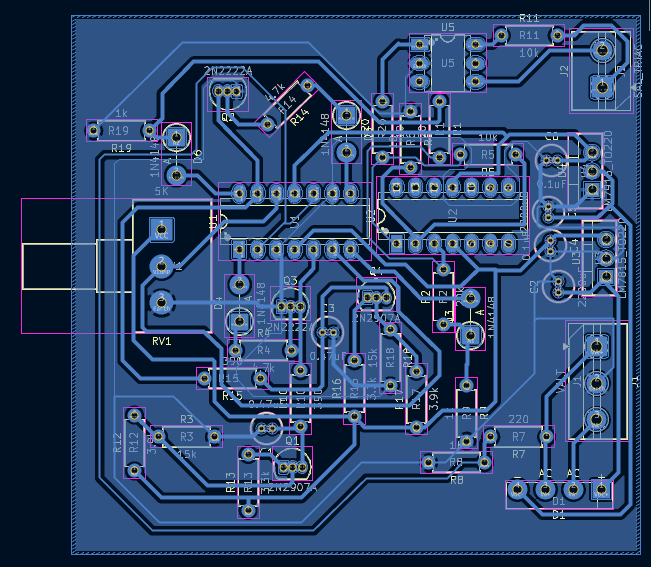
\includegraphics[width=0.8\linewidth]{AC/EXKicad.png}
     \caption{Diseño del PCB en KiCad.}
     \label{fig:kicad}
 \end{figure}
\subsection{Validación mediante Simulación}
 
Antes de la construcción física, se realizó una simulación completa del circuito utilizando Orcad SPICE. Se modelaron detalladamente las etapas 2, 3 y 4, mientras que las etapas 1 y 5 fueron de implementación estándar. Los resultados de simulación validaron la operación del sistema bajo diferentes condiciones de ángulo de disparo.

A continuación, se presenta la simulación realizada en LTSpice en la Figura~\ref{fig:sim}. En la Figura~\ref{fig:onda} se muestran las formas de onda obtenidas, donde se aprecia la modulación PWM de la salida.
 
\begin{figure}[!h]
     \centering
    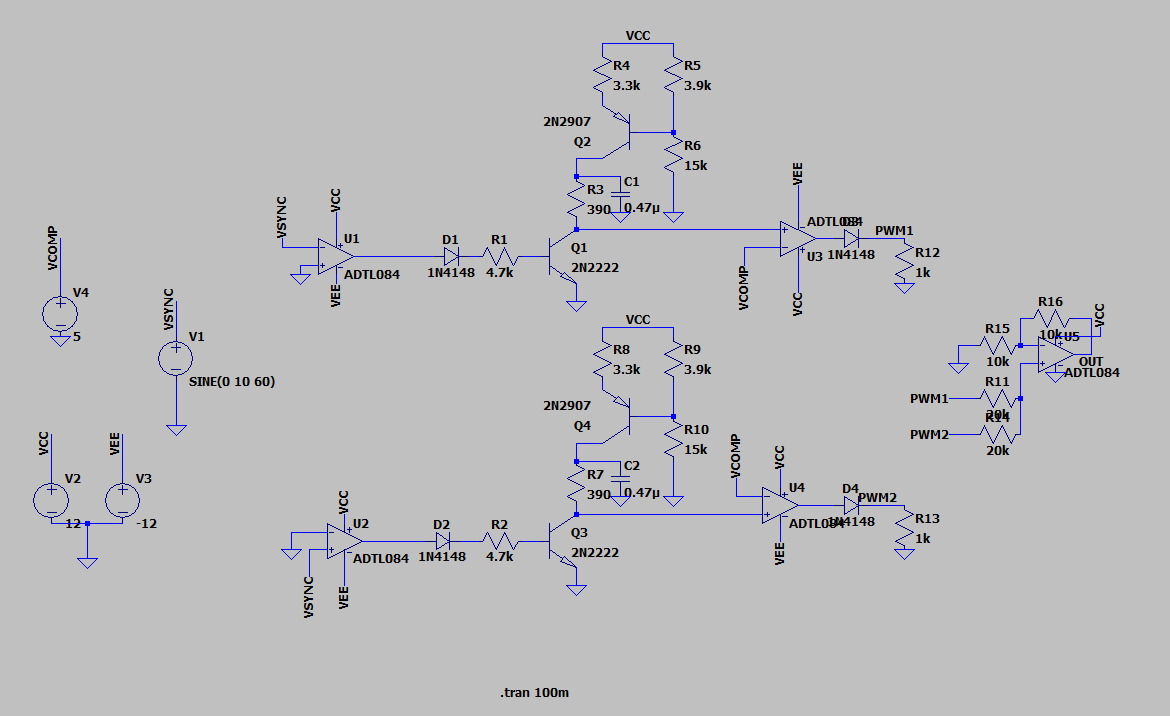
\includegraphics[width=0.8\linewidth]{AC/Simulacion.png}
    \caption{Esquemático en LTSpice.}
     \label{fig:sim}
 \end{figure}


 \begin{figure}[!h]
     \centering
     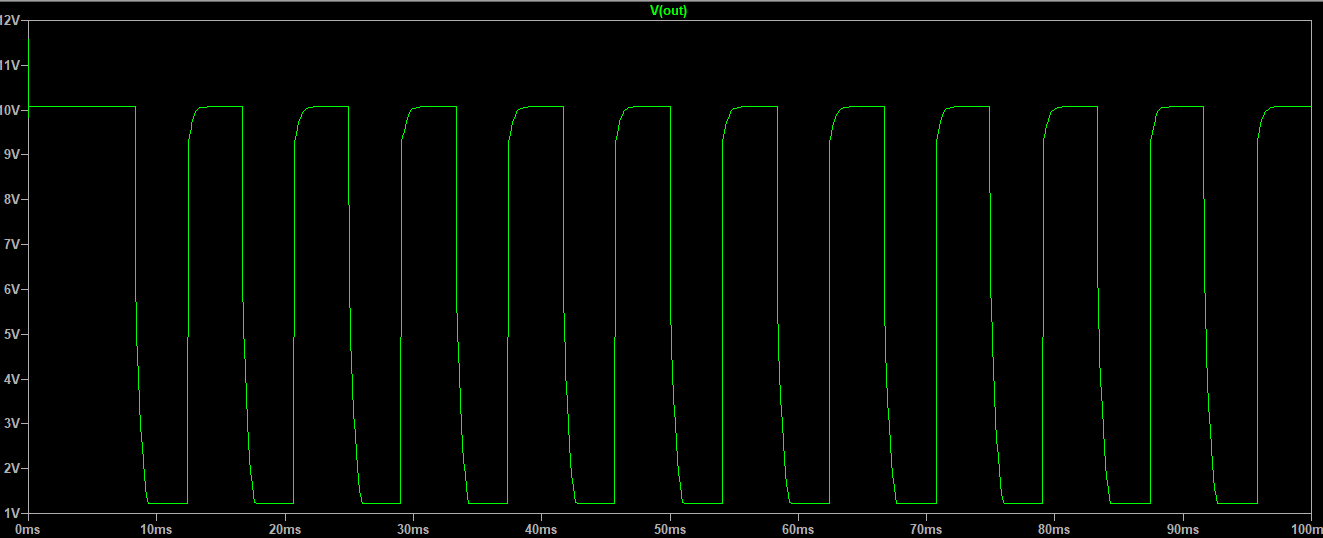
\includegraphics[width=0.8\linewidth]{AC/salida.png}
     \caption{Salida obtenida en simulación.}
     \label{fig:onda}
 \end{figure}


 \newpage 
 
\subsection{Validación Experimental}
 
Una vez completada la construcción del prototipo, se procedió a validar experimentalmente el funcionamiento mediante mediciones con osciloscopio, comparando los resultados con las predicciones teóricas y simuladas, tal como se muestra en la Figura~\ref{fig:out}.
 
 
\begin{figure}[!h]
     \centering
    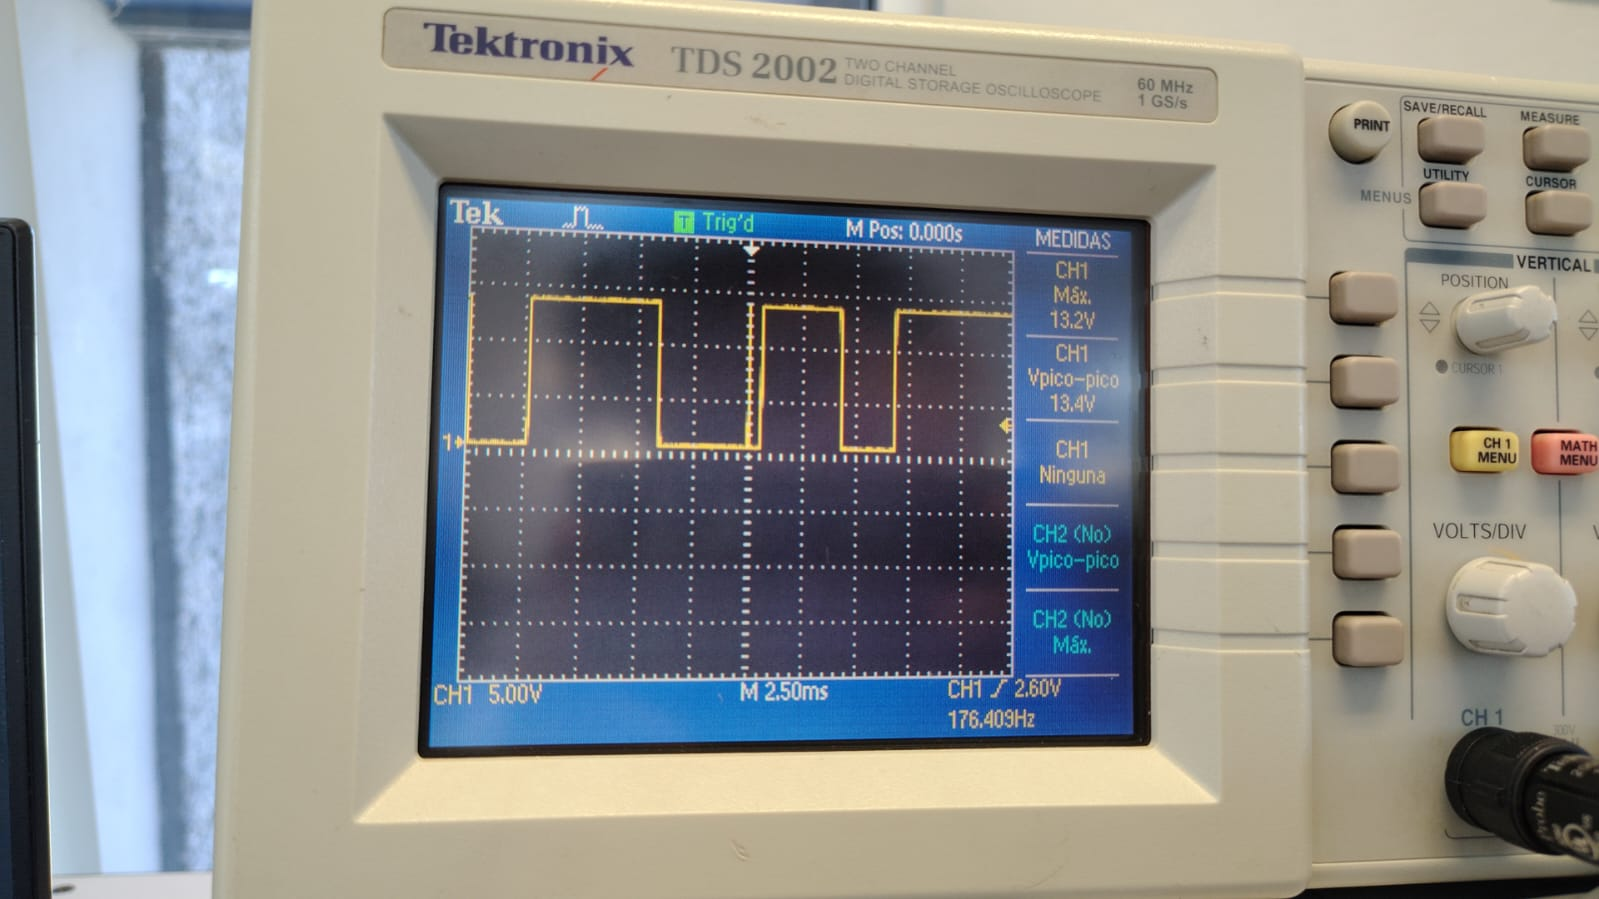
\includegraphics[width=0.85\linewidth]{AC/Salida.png}
     \caption{Formas de onda obtenidas en pruebas experimentales.}
     \label{fig:out}
 \end{figure} 


\section{Discusión}

La TDC permite un control de $0^{\circ}$ a $180^{\circ}$, con alta precisión, aislamiento eléctrico completo, operación a voltajes de red y simetría en ambos semiciclos. Es fundamental seleccionar correctamente la capacitancia y usar componentes de precisión. Desde la perspectiva educativa, permite al estudiantado construir un sistema complejo al aplicar teoría directamente. En comparación con otras soluciones, la TDC ofrece mayor flexibilidad y funcionalidad, aunque a costa de mayor complejidad de diseño y construcción.

El diseño de esta placa representó un desafío significativo debido a diversos inconvenientes técnicos que surgieron durante el desarrollo. Uno de los problemas más relevantes fue el ancho de las pistas, lo que dificultó la integración de todas las etapas en un solo PCB. Para superar este desafío, se realizaron múltiples iteraciones del diseño, ajustando el layout para optimizar el espacio y garantizar una separación adecuada entre las etapas de control y potencia.

\section{Reflexiones Personales}
\subsection*{Contreras Reyes Orlando}
Este proyecto me resultó interesante, debido a que me permitió aplicar conocimientos teóricos en un proyecto práctico. Sin embargo, enfrenté dificultades técnicas durante el diseño del PCB, lo que me enseñó la importancia de la planificación y la iteración en el proceso de diseño. A pesar de los desafíos, la experiencia fue enriquecedora y me permitió desarrollar habilidades valiosas en electrónica de potencia. Lo que nos atrasó mucho fue el diseño del PCB, ya que tuvimos que hacer varios diseños debido al ancho de las pistas y la necesidad de mantener una separación adecuada para evitar cortocircuitos, especialmente en la etapa de potencia. Sin embargo, esta experiencia me enseñó la importancia de la paciencia y la perseverancia en el proceso de diseño, así como la necesidad de considerar cuidadosamente el layout desde el principio para evitar problemas posteriores.


Siento que el proceso más tedioso o donde fue el cuello de botella del proyecto fue la creación de la placa, considero que si se tuviera cubierta esa parte de una forma menos artesanal facilitaría mucho el proceso, personalmente no veo la necesidad de hacerlo de forma artesanal, ya que existen servicios de fabricación de PCB que pueden producir placas de alta calidad a un costo razonable y esto permitiría a los estudiantes centrarse en placas más complejas y funcionales, en lugar de dedicar tiempo a la fabricación manual de placas, lo que puede ser propenso a errores y consume mucho tiempo.


La parte de diseño personalmente me encantó, en general me gusta el diseño de esquemáticos y PCBs, siento que algo que pudiera aplicarse es que nosotros realizáramos el diseño del PCB pero que se mandara a fabricar, esto nos permitiría centrarnos más en el diseño y la funcionalidad de la placa, en lugar de dedicar tiempo a la fabricación manual, lo que puede ser propenso a errores y consume mucho tiempo. Además, esto nos permitiría experimentar con diseños más complejos y funcionales, lo que enriquecería aún más nuestra experiencia de aprendizaje.
\newpage

\subsection*{García Barrera Iker Emiliano}
Este examen práctico fue una experiencia muy enriquecedora, ya que me permitió aprender a utilizar los amplificadores operacionales (op-amps), realizar cálculos de valores y comprender mejor cómo se llevan a cabo las pruebas dentro de un diseño. También entendí de manera más clara cómo se desarrolla un circuito desde su planeación hasta su implementación.
Además, este examen práctico me dejó aprendizajes importantes en el trabajo en equipo. Aprendí a delegar tareas, a organizar tiempos y a entender que no todo funciona a la primera, por lo que es necesario tener perseverancia y paciencia durante el proceso.
En cuanto a las dificultades, considero que tuvimos ciertas complicaciones, principalmente relacionadas con las pistas (venas) y el diseño de la placa PCB. Esto se debe a que aún no tenemos mucha experiencia en la elaboración de placas, por lo que es un aspecto que definitivamente necesitamos reforzar. Sin embargo, considero que fue muy valioso enfrentarnos a estos problemas, ya que nos permitió identificar deficiencias que de otra forma habríamos seguido arrastrando.
También se presentaron retos durante el proceso de fabricación, como el manejo del ácido y la elaboración de la placa fenólica de cobre. Estas dificultades no solo representaron un obstáculo, sino que también se convirtieron en una oportunidad de aprendizaje.

A partir de esto, en lo personal, me surgió una motivación importante: explorar alternativas como el uso de una fresadora o CNC para la fabricación de placas, lo que permitiría hacer prototipos de manera más rápida, precisa y automatizada. Considero que esta idea es uno de los aprendizajes más valiosos que me dejó este proyecto.


En el aspecto humano, considero que fue una experiencia muy valiosa. Estoy muy agradecido con mis compañeros de equipo, ya que demostraron constancia y dedicación en todo momento. Aprendí a confiar en ellos, y no solo cumplieron con lo esperado, sino que superaron mis expectativas, lo cual valoro mucho.
En cuanto a los conocimientos técnicos, reforcé el uso de op-amps en distintas configuraciones, así como el funcionamiento de los optoacopladores. Siento que este proyecto representó un nivel más avanzado en comparación con los semestres anteriores, ya que logramos integrar una fuente de poder junto con el circuito completo en una misma placa.
Finalmente, considero que este proyecto nos permitió acercarnos más a un entorno real, ya que el resultado obtenido podría adaptarse fácilmente a una aplicación práctica, como parte de un módulo dentro de una maquinaria más grande. En general, pienso que el proyecto estuvo muy bien alineado con los objetivos de la materia y aportó tanto en lo técnico como en lo personal.

\subsection*{Lara Hernández Kevin Adrián}
Este proyecto de examen me resultó en una mezcla de distintas experiencias y emociones que viví y aprendí a lo largo del proceso de fabricación del PCB y del circuito en general. Cuando comenzamos, me pareció sencillo y considero que dar por hecho que se terminaría de manera rápida fue uno de los errores que tal vez nos llevó, a mi equipo y a mí, no solo a no lograr a tiempo un buen funcionamiento del circuito, sino también a una profunda frustración con el resultado. Es claro que uno de los mayores problemas durante el proceso de realización del control de disparo fue la falta de planificación adecuada de algunos tiempos; quizá, si se hubiese tomado más tiempo para probar las etapas de manera más detallada, se habrían podido corregir errores que nos costaron tiempo y esfuerzo. En primer lugar, los esquemáticos fueron deficientes en varios puntos y, con el tiempo encima por una mala planificación, dichos problemas se tuvieron que resolver al momento de la fabricación del PCB mediante cables y distintas modificaciones que pudieron haber contribuido a la inestabilidad de algunas partes del circuito. Fue extremadamente tedioso soldar y remover soldadura de componentes que, por el método de fabricación, tenían pads frágiles y alta probabilidad de fallar o romperse, ocasionando tener que fabricar de nuevo el PCB. Esa fue, a mi parecer, la parte más tediosa y que, con una buena planificación desde un inicio, habría sido más sencilla de corregir o evitar.


Pienso que de todo esto aprendí dos grandes cosas más allá del apartado técnico: mejorar los tiempos de organización con mi equipo y, la segunda, que considero la más importante, no subestimar un proyecto porque aparente ser relativamente sencillo. El exceso de confianza, o quizá no prever posibles escenarios desfavorables, ha sido uno de los errores más repetidos a lo largo de nuestra historia como seres humanos. Aunque probablemente no sea un tema de relevancia existencial, me deja reflexionando sobre todo esto, y creo que, al final de cuentas, esa es la parte más importante de cometer un error: aprender y que ese aprendizaje sea valioso para que no se repitan los errores o, si se repiten, que no sea con la misma gravedad de consecuencias. Lo más valioso de todo esto, además de la lección aprendida sobre el exceso de confianza, fue el entendimiento de este proyecto: cómo los tiristores son fundamentales para la corriente alterna. Aunque no haya resultado de manera perfecta al final, entender por qué funciona este circuito y, más importante, cómo funciona, es muy valioso y deja pensando en que los controles de potencia en corriente alterna, y en general los tiristores como dispositivos, son fundamentales en cómo funcionan muchas partes del mundo en el que vivimos.
\newpage

\subsection*{Jiménez de Luna Rafael Odín}
Más allá de que este proyecto correspondiente al primer parcial representaba la principal prioridad de la materia, considero que también fue una excelente oportunidad para fortalecer habilidades que van más allá del conocimiento técnico, especialmente en lo relacionado con el trabajo en equipo. Esta actividad me permitió comprender, más que nunca, la importancia de una buena comunicación entre los integrantes del grupo, así como la correcta asignación de roles. Si bien todos aportamos el mismo empeño y compromiso durante el desarrollo, cada integrante asumió responsabilidades distintas acorde a sus habilidades, lo cual facilitó el avance del proyecto. Esto me llevó a valorar profundamente la relevancia del trabajo colaborativo como una de las principales enseñanzas, ya que no solo se trata de dividir tareas, sino de integrar esfuerzos de manera efectiva para lograr un objetivo común.

Asimismo, me gustaría destacar la importancia de la aplicación de la Electrónica de Potencia en este examen/proyecto, ya que permitió aterrizar conceptos teóricos en una situación más cercana a la realidad. El hecho de trabajar con dispositivos y circuitos con posibles aplicaciones prácticas le da un sentido mucho más significativo al aprendizaje adquirido durante el parcial. Esto no solo refuerza los conocimientos vistos en clase, sino que también despierta un mayor interés por la materia, al poder visualizar su utilidad en contextos reales. Además, este tipo de evaluaciones fomenta el desarrollo del pensamiento crítico, ya que es necesario analizar, probar y corregir constantemente hasta lograr un funcionamiento adecuado.

Por otro lado, es importante mencionar que, a pesar de las dificultades que enfrentamos a lo largo del desarrollo del proyecto, estas también representaron oportunidades importantes de aprendizaje. Uno de los principales aspectos a mejorar fue la gestión del tiempo, ya que en distintos momentos el avance se vio limitado por una planeación poco eficiente. Considero que una mejor organización desde el inicio, así como una distribución más estratégica de las tareas, habría permitido optimizar recursos y reducir errores. Aun así, el hecho de enfrentar estos retos nos ayudó a desarrollar habilidades de resolución de problemas y a mantener una actitud resiliente ante las adversidades, lo cual resulta fundamental en la formación académica y profesional.

Finalmente, puedo concluir que este examen/proyecto del primer parcial no solo contribuyó a reforzar mis conocimientos en el área de la Electrónica de Potencia, sino que también me permitió desarrollar habilidades personales y de trabajo en equipo que serán de gran utilidad en futuros proyectos académicos. A pesar de que el resultado no fue exactamente como se había planeado en un inicio, me siento satisfecho con el aprendizaje obtenido y con el esfuerzo colectivo realizado. Sin duda, esta experiencia deja una base sólida tanto en lo técnico como en lo humano, aspectos esenciales en la formación como ingeniero.
\begin{thebibliography}{99}

\bibitem{ref1}
ALF. ``Dimmer digital utilizando un microcontrolador PIC''. Microcontroladores y Software. Consultado: junio de 2015.

\bibitem{ref2}
Boylestad, R. L., \& Nashelsky, L. (2003). \textit{Dispositivos pnpn y otros}. En Electrónica: teoría de circuitos y dispositivos electrónicos (pp. 923-964). Pearson, Prentice Hall.

\bibitem{ref3}
Hayt, W. H., Kemmerly, J. E., \& Durbin, S. M. (2012). \textit{Capacitores e inductores}. En Análisis de circuitos en ingeniería (pp. 217-260). Mc Graw Hill.

\bibitem{ref4}
Control de potencia en alterna. (2011). \textit{Prácticas de laboratorio}. Escuela Técnica Superior de Ingenieros Industriales ETSII, Universidad Politécnica de Madrid.



\bibitem{ref7}
Malvino, A., \& Bates, J. B. (2007). \textit{Tiristores}. En Principios de Electrónica (pp. 490-529). Mc Graw Hill.

\bibitem{ref8}
Wildi, T. (2007). \textit{Elementos fundamentales de electrónica de potencia}. En Máquinas eléctricas y sistemas de potencia (pp. 480-554). Pearson, Prentice Hall.

\end{thebibliography}

\end{document}